% What kind of text document should we build
\documentclass[a4,10pt]{article}


% Include packages we need for different features (the less, the better)

% Clever cross-referencing
\usepackage{cleveref}

% Math
\usepackage{amsmath}

% Algorithms
\usepackage{algorithm}
\usepackage{algpseudocode}

% Tikz
\RequirePackage{tikz}
\usetikzlibrary{arrows,shapes,calc,through,intersections,decorations.markings,positioning}

\tikzstyle{every picture}+=[remember picture]

\RequirePackage{pgfplots}









% Set TITLE, AUTHOR and DATE
\title{Simple Go With C++ Programming}
\author{Jiaxin Lin}
\date{\today}
 


\begin{document}



  % Create the main title section
  \maketitle

  \begin{abstract}
    This article presents a simple Go game in c++ programming.
    Update the program,and using the program can play go game,it has some basic and simple functinon such as:
    basic ko rules ,suicide rules,capturing the stone.Using the environment of computer go program,
    matching with the recursion algorithm.
     \end{abstract}


  %%%%%%%%%%%%%%%%%%%%%%%%%%%%%%%%%%%%%%
  %%  The main content of the report  %%
  %%%%%%%%%%%%%%%%%%%%%%%%%%%%%%%%%%%%%%
 
  \section{Introduction}



      Go is a puzzle game originated in China, first tell us about the basics of chess:
      , Pieces of gas, means: a piece on the board,
      and it is a straight line close to the null point of this piece of "gas" meas the freedom.
      Straight line next to the piece points, if there is the same color pieces exist,
      they will be interconnected into an integral whole. Their gas should also be calculated.

       Grapes, refers to as a chess all the other gas are occupied, it was no gas in the state, will be put off, known as "grapes."
       If erupted after the two sides were tested piece airless state, no gas should only extract the other son.\cite{he:2009}(see \cref{fig:lena}).
      \begin{figure}[tbp]
      \centering
     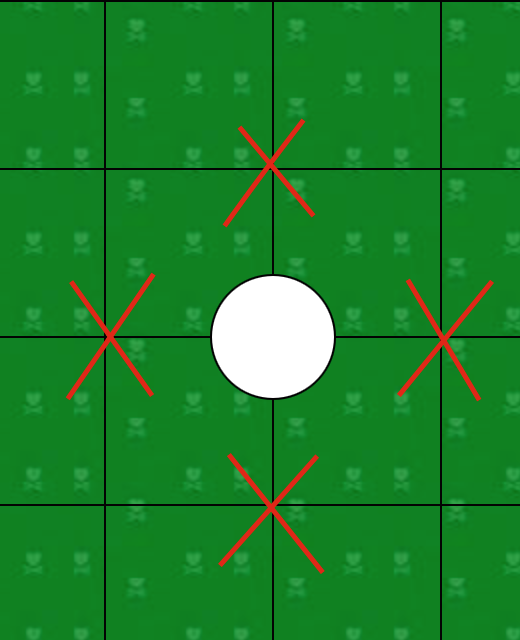
\includegraphics[width=0.30\textwidth]{gfx/gas.png}
     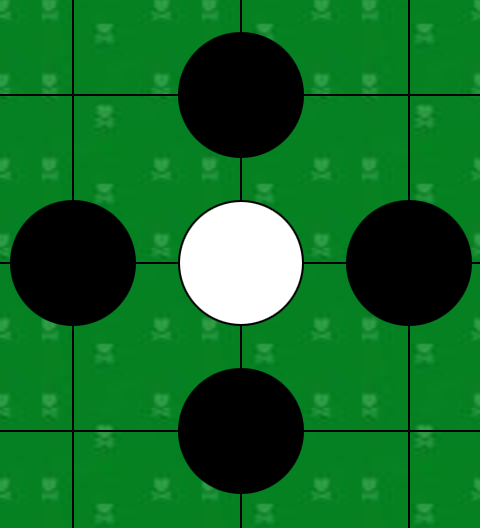
\includegraphics[width=0.30\textwidth]{gfx/nogas.png}
     \caption{The White 4 freedoms and no freedom }
     \label{fig:lena}
     \end{figure}


  \section{Methods of capture}
    Recursion in computer science is a method where the solution to a problem depends on solutions to smaller instances of the \texttt{same problem}.
    When only one stone is easy to know the freedoms,but in some stones need to think how to caculate the freedoms.\cite{Graham:1990}(see \cref{fig:freedoms}).
    So need to use recursion to deal with this.First should already calculate the place first stone then judge the west weather have stones,same color,calculate the freedoms.
    if the west no stone and haven't calculate the freedoms then the number of freedoms plus one and make a sign of this empty
    space have been calculate the freedoms.else if the west have stone and same color and haven't calculate the freedoms then
    recursive call to the east point.In the way can search the next stones like east,north and south.

      \begin{figure}[tbp]
      \centering
     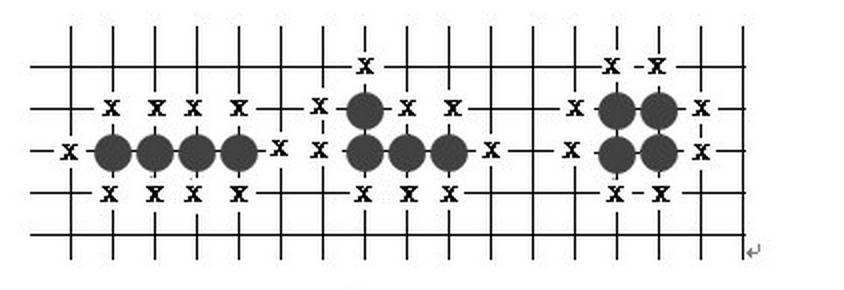
\includegraphics[width=0.40\textwidth]{gfx/freedoms.png}
     %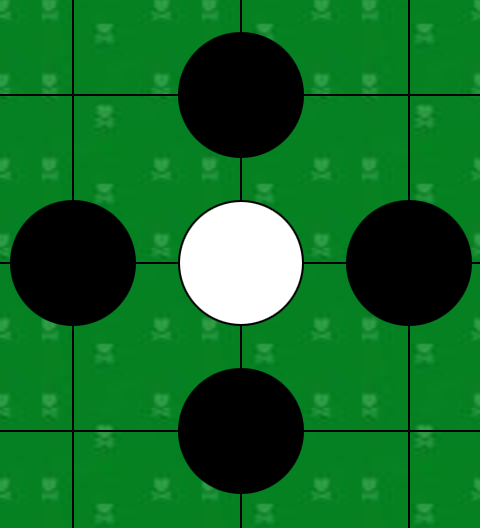
\includegraphics[width=0.30\textwidth]{gfx/nogas.png}
     %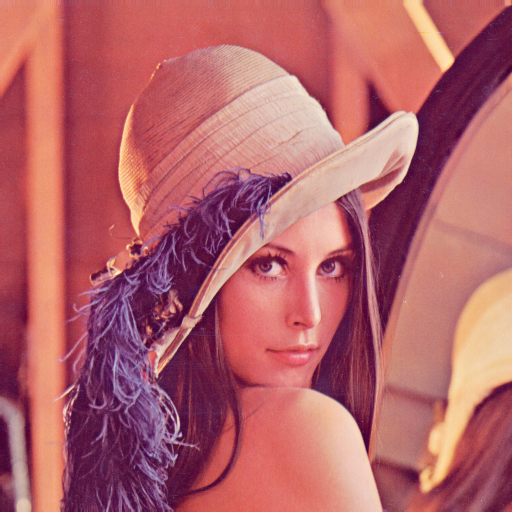
\includegraphics[width=0.30\textwidth]{gfx/lena.png}
     \caption{ 4 stones with different freedom values}
     \label{fig:freedoms}
     \end{figure}

    Then can calculate a block of stones freedoms.Use of for loop to search the whole board
    return the calculate freedom numbers.

    Finially can remove means capture the stones.Need to follow the stone no freedoms and different color.




%\begin{itemize}
%      \item Add a short description of the O-notation (with a reference to Knuth's paper from 1976)\footnote{Hint: ``Big Omicron and Big Omega and Big Theta''.}.
%      \item Recall that the O-notation enables us to describe an algorithm's response to variation of the size of the input data.
%    \item Mathematics can either be placed in the text, such as $f(x)=\frac{1}{x}$, or as equations:
%    \end{itemize}
%    \begin{equation}
%      \label{eq:integral}
%      f(x) = \int_{-\infty}^{\infty}\frac{sin(x)}{x}dx.
%    \end{equation}
%    \begin{itemize}
%      \item Equations can be referred to. The RHS of formula \eqref{eq:integral} is a well-known indefinite integral. A plot of $\frac{sin(x)}{x}$ is provided in \cref{fig:plot_function}.
%    \end{itemize}

% \begin{figure} %[width=\textwidth]
%   \begin{tikzpicture}
%     \begin{axis}[
%       xmajorgrids=false,ymajorgrids=false,
%       legend pos=north east,
%       width=0.9\textwidth, height=0.25\textheight,
%        reverse legend
%       ]
%
%       \addplot[blue,domain=-25.1:25.1,samples=500] {sin(deg(x))/x};
%       \legend{
%         $\frac{sin(x)}{x}$
%       }
%     \end{axis}
%   \end{tikzpicture}
%   \caption{A plot of the function $\frac{sin(x)}{x},$ for $x \in [-25.1,25.1]$.}
%   \label{fig:plot_function}
% \end{figure}
    
         \begin{figure}[tbp]
         \centering
        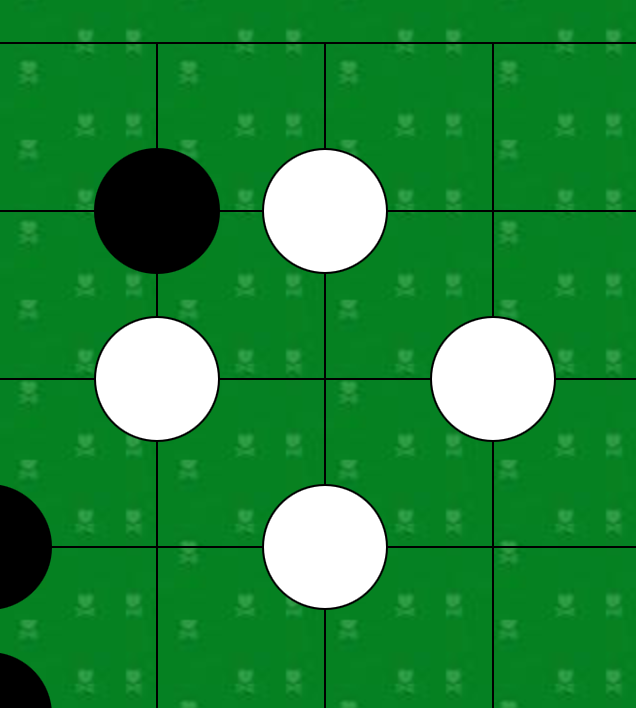
\includegraphics[width=0.30\textwidth]{gfx/suicide.png}
        %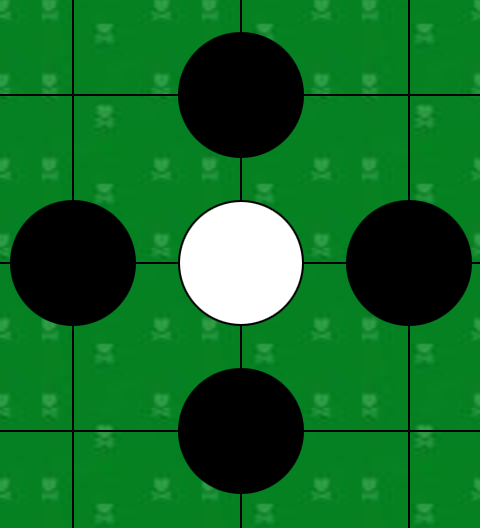
\includegraphics[width=0.30\textwidth]{gfx/nogas.png}
        %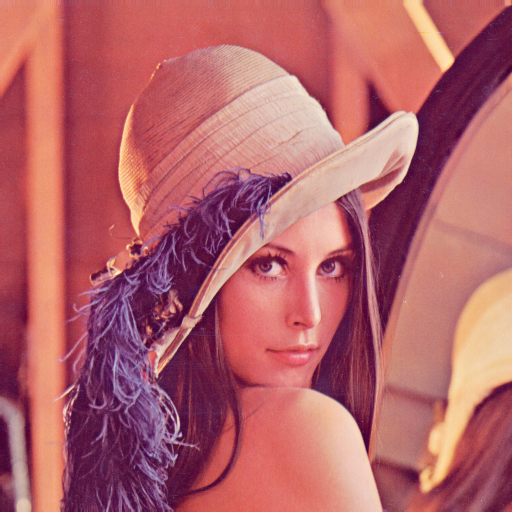
\includegraphics[width=0.30\textwidth]{gfx/lena.png}
        \caption{The black stone not allowed to place inside}
        \label{fig:suicide}
        \end{figure}
  \section{Methods of suicide}
Though in most positions suicide is an obvious bad move, there exist positions where suicide could be used as a ko threat.
In such cases it can be argued that suicide adds something to the game. A drawback of allowing suicide is that the length of the game can increase drastically if players are unwilling to pass (and admit defeat). In most rule sets (Japanese, Chinese, North American, etc.)
suicide is not allowed (British Go Association, 2001). So, in all our experiments suicide is illegal.\cite{werf:2003}(see \cref{fig:suicide}).

In order to achieve this function just make the stones not allowed to place in the position's freedom equals null.Then
not change the player(color).Use the for loop to search where position not allowed.
% \begin{itemize}
%   \item Describe briefly the bubble sort algorithm (a reference or two to any standard text book on algorithms would be in order).
%   \item Don't forget to mention Bubble sort's performance using the O-notation.
% \end{itemize}

        \begin{figure}[tbp]
         \centering
        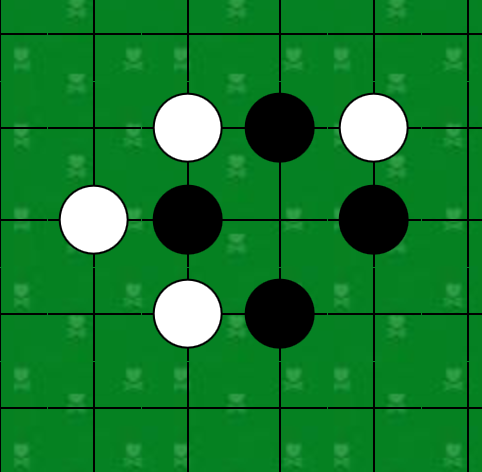
\includegraphics[width=0.30\textwidth]{gfx/ko.png}
        %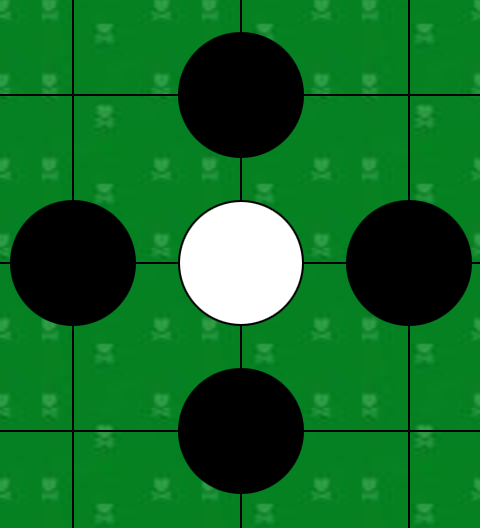
\includegraphics[width=0.30\textwidth]{gfx/nogas.png}
        %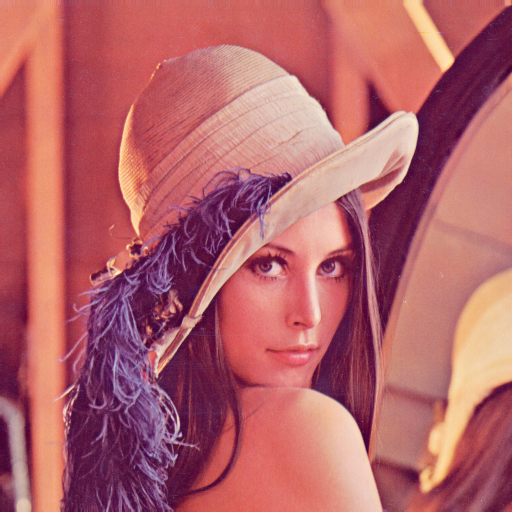
\includegraphics[width=0.30\textwidth]{gfx/lena.png}
        \caption{show ko  }
        \label{fig:ko}
        \end{figure}
  \section{Methods of BasicKo}
  Since stones can be captured (and removed from the board) it is possible to repeat previous board positions.
  However, infinite games are not practical, and therefore repetition of positions should be avoided.
  The most common case of a repeating position is the basic ko.\cite{werf:2003}(see \cref{fig:ko}).

The basic-ko rule says that direct recreation of a previous board position in a cycle of two moves is forbidden.
As a consequence White can only recapture the black stone after playing a threatening move elsewhere which changes the whole-board position. Such a move is called a ko threat.

In order to achieve this function need to save the previous step.If the place stone's position are same and color still same need
to place other where.

%    In \cite{shell:1959} Shell introduced a high-speed sorting procedure.
%    It has later become known as \emph{Shell sorting}.
%    \begin{itemize}
%      \item Complete the short description of Shell's sorting algorithm.
%      \item Use the example algorithm listing environment below as a starting point.
%    \end{itemize}
%    \begin{algorithm}
%      \caption{Euclid's algorithm}\label{euclid}
%      \begin{algorithmic}[1]
%        \Procedure{Euclid}{$a,b$}\Comment{The g.c.d. of a and b}
%        \State $r\gets a\bmod b$
%        \While{$r\not=0$}\Comment{We have the answer if r is 0}
%        \State $a\gets b$
%        \State $b\gets r$
%        \State $r\gets a\bmod b$
%        \EndWhile\label{euclidendwhile}
%        \State \textbf{return} $b$\Comment{The gcd is b}
%        \EndProcedure
%      \end{algorithmic}
%    \end{algorithm}

  \section{Results}
  Describe how the benchmark was performed. Be objective - don't describe too many details.
  The reader which this text is meant for should be able to reconstruct the experiment using his own tools.
  Some examples of topics for this section:
    \begin{itemize}
      \item The capture of stones
      \item The suicide
      \item The basic Ko rules
      \item Change the backround of board and word style
      \item Calculate the score just calculate the stones on the board in different color
      \end{itemize}

  \section{Discussion}
About calculate the score is a difficult problems.Ask for Someone who can play go well.Recognizing the Go is not easy to judge which
one win.And I know why need to creat the boundary.It will easy to calculate by each modular.
Judge which player are winner need to finish all the stones.(see \cref{fig:finish})Then need to judge the stone who are
life or death.Because during the game is unpredictable.And the score rules devide Chinese and Janpanese.For the Janpanese is more
need to caculate the positon of empty in the board and died stone need to calculate twice.


About the recursion algorithms are more suitable for a small board, if size increase is not very appropriate.
Need to find a better way to calculate. But now the recursion algorithm is easy to think to solve this problem.


        \begin{figure}[tbp]
         \centering
        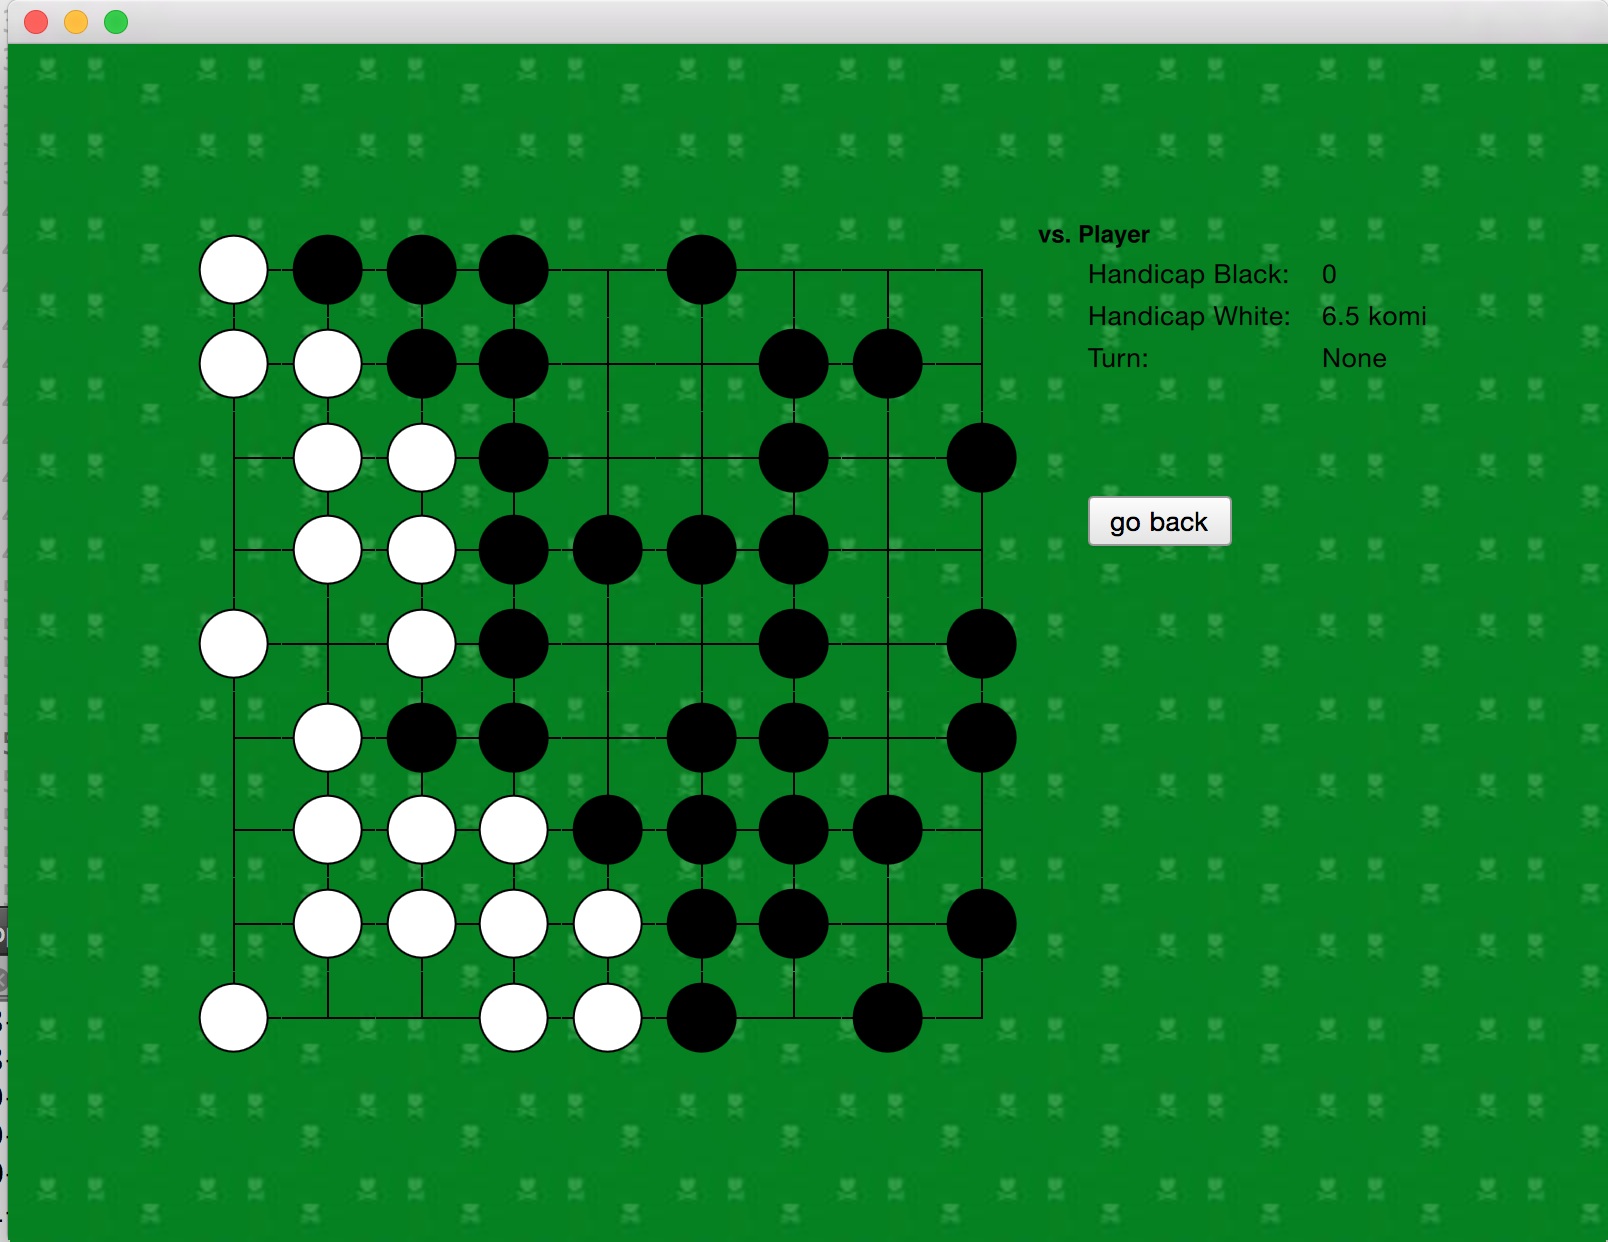
\includegraphics[width=0.80\textwidth]{gfx/finish.png}
        %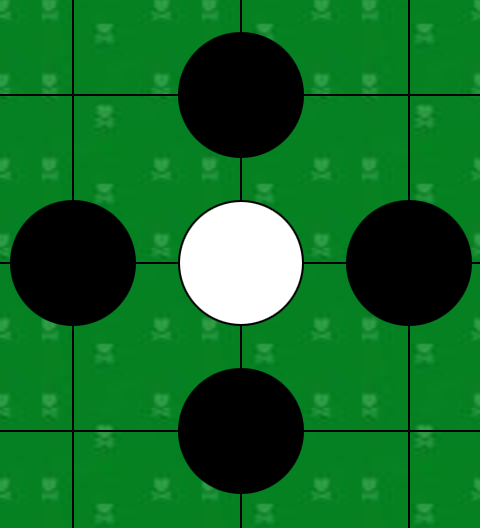
\includegraphics[width=0.30\textwidth]{gfx/nogas.png}
        %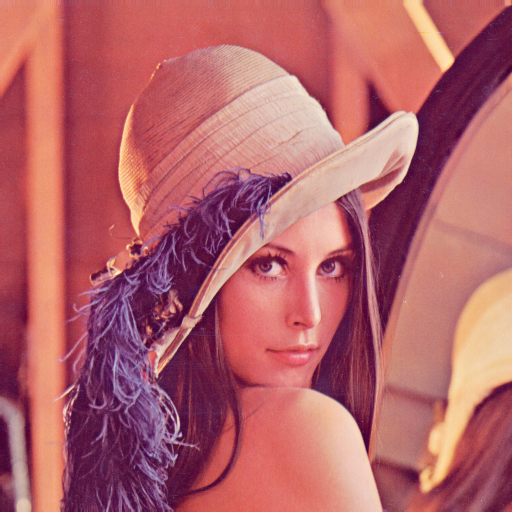
\includegraphics[width=0.30\textwidth]{gfx/lena.png}
        \caption{The ending of go  }
        \label{fig:finish}
        \end{figure}

%    A graphical visualization of bytes allocated vs. allocation time in milliseconds for the vector benchmark is shown in \cref{fig:bench_vector}.
%
%    \begin{figure}%[width=\textwidth]
%      \begin{tikzpicture}
%        \begin{axis}[
%          xmajorgrids=false,ymajorgrids=false,
%          legend pos=south east,
%          width=0.9\textwidth, height=0.25\textheight,
%%          reverse legend
%          ]
%
%          \addplot[red] table[x=size ,y=time, skip first n=0] {dat/benchmark_vector_stl.dat};
%          \addplot[blue] table[x=size ,y=time, skip first n=0] {dat/benchmark_vector_reserve.dat};
%          \legend{
%            STL,
%            mylib
%          }
%        \end{axis}
%      \end{tikzpicture}
%      \caption{Run-times: \emph{milliseconds} to allocate and construct number of objects * sizeof(int) \emph{bytes} of data.}
%      \label{fig:bench_vector}
%    \end{figure}
%
%    \Cref{fig:bench_sort} shows performance graphs for the Bubble- and Shell sorting algorithms, together with STL's \texttt{sort()} for reference, measured in milliseconds for some predefined numbers of items.
%
%    \begin{figure}%[width=\textwidth]
%      \begin{tikzpicture}
%        \begin{axis}[
%          xmajorgrids=false,ymajorgrids=false,
%          legend pos=north west,
%          width=0.9\textwidth, height=0.25\textheight,
%%          reverse legend
%          ]
%
%          \addplot[green] table[x=size ,y=time, skip first n=0] {dat/benchmark_stl_sort.dat};
%          \addplot[red] table[x=size ,y=time, skip first n=0] {dat/benchmark_mylib_bubble.dat};
%          \addplot[blue] table[x=size ,y=time, skip first n=0] {dat/benchmark_mylib_shell.dat};
%          \legend{
%            STL sort,
%            bubble,
%            Shell
%          }
%        \end{axis}
%      \end{tikzpicture}
%      \caption{Run-times: \emph{milliseconds} to sort number of objects.}
%      \label{fig:bench_sort}
%    \end{figure}
%
%  \section{Concluding remarks}
%  \begin{itemize}
%    \item Reflect over the method and results.
%    \item Topics for future work could be suggested here.
%  \end{itemize}
%  Example: By comparing the performance of the reserve and emplace functionality of the STL version of the vector to our custom vector implementation from \emph{mylib} we conclude that the STL vector is slightly faster at the specified operation.



  % Include the bibliography
  \bibliographystyle{plain}
  \bibliography{bibliography}

\end{document}
